\documentclass[12pt%
%,draft%
,aspectratio=169%
]{beamer}
%
\usepackage{fontspec}
\defaultfontfeatures{Ligatures=TeX}
%\setsansfont{Liberation Sans}
\usepackage{polyglossia}
\setdefaultlanguage{ngerman}
% Alternative template for talks of the Freie Universität Berlin.
% Created by Leonard R. König, <leonard.koenig@fu-berlin.de> following the
% guidelines on www.fu-berlin.de/cd
%
% (c) Leonard König, CC BY 4.0
%
% This template was written against UTF-8 capable LaTeX engines, specifically
% LuaLaTeX.

% Trying to get rather close to the ppt/odp template:
%  http://www.fu-berlin.de/sites/cd/downloads_container/PowerPoint_Praesentation_Anleitung.pdf

%%% font styles
\setbeamerfont{frametitle}{series=\bfseries}
\setbeamerfont{footline}{series=\bfseries}
\setbeamerfont{headline}{series=\bfseries}
\setbeamerfont{alerted text}{series=\bfseries}
%%%

% colordefs
\definecolor{fu_darkblue}{RGB}{0,51,102}
\definecolor{fu_seablue}{RGB}{0,102,204}
\definecolor{fu_lightblue}{RGB}{204,214,224}
\definecolor{fu_green}{RGB}{153,204,0}
\definecolor{fu_lightgrey}{RGB}{128,128,128}
\definecolor{fu_grey}{RGB}{95,95,95}
%
\definecolor{fu_red}{RGB}{204, 0, 0} % red text (used by \alert)
%%% end colordefs

%%% colors
\setbeamercolor*{title}{fg=fu_darkblue}
\setbeamercolor*{subtitle}{fg=fu_seablue}
\setbeamercolor*{frametitle}{fg=fu_darkblue}
\setbeamercolor*{footline}{fg=fu_grey,bg=fu_lightblue}
\setbeamercolor*{headline}{fg=fu_grey}

\setbeamercolor*{normal text}{fg=black}
\setbeamercolor*{alerted text}{fg=fu_red}
\setbeamercolor*{example text}{fg=fu_green}
\setbeamercolor*{structure}{fg=fu_darkblue}

\setbeamercolor*{block title}{fg=white,bg=black!50}
\setbeamercolor*{block title alerted}{fg=white,bg=black!50}
\setbeamercolor*{block title example}{fg=white,bg=black!50}

\setbeamercolor*{block body}{bg=black!10}
\setbeamercolor*{block body alerted}{bg=black!10}
\setbeamercolor*{block body example}{bg=black!10}

\setbeamercolor{bibliography entry author}{fg=fu_darkblue}

\setbeamercolor{item}{fg=fu_darkblue}
\setbeamercolor{navigation symbols}{fg=fu_lightgrey,bg=fu_grey}
%%% end colors

%%% title page
% Display logo (if exists) and right next to it, put our title + subtitle
\defbeamertemplate*{title page}{fu_titlepage}
{%
	\hskip .3\textheight
	\begin{minipage}[.4\textheight]{\textwidth}
		\begin{minipage}[.4\textheight]{0.25\textwidth}
			\inserttitlegraphic
		\end{minipage}%
		\begin{minipage}[.4\textheight]{0.75\textwidth}
			\begin{beamercolorbox}{title}
				\usebeamerfont{title}\inserttitle\par%
			\end{beamercolorbox}
			\vfill
			\ifx\insertsubtitle
				\@empty%
			\else
				\begin{beamercolorbox}{subtitle}
					\usebeamerfont{subtitle}\insertsubtitle\par
				\end{beamercolorbox}
			\fi
		\end{minipage}
	\end{minipage}%
	\hskip .3\textheight
}
%%% end title page

%%% headline
% display title, author and institute on the left;
% logo on the right.
\newcommand{\headlinetext}
{%
	\inserttitle\\[0.3em]%
	\insertauthor, %
	\insertshortinstitute
}
\newlength{\headlinewidth}
\setlength{\headlinewidth}{\paperwidth}
\addtolength{\headlinewidth}{-2\marginparsep}
\setbeamertemplate{headline}
{%
	\begin{beamercolorbox}[wd=\paperwidth]{headline}%
		\vskip5pt
		{\hspace*{\marginparsep}}%
		\parbox{.5\headlinewidth}
		{%
			\usebeamertemplate{title in head/foot}%
			\headlinetext%
		}%
		\begin{minipage}{.5\headlinewidth}%
			\hfill\usebeamertemplate*{logo}
		\end{minipage}%
		{\hspace*{\marginparsep}}%
	\end{beamercolorbox}%
}
%%% end headline

%%% footline
% title + date on the left, frame number on the right
\newcommand{\footlinetext}
{%
	\usebeamerfont{shorttitle}\insertshorttitle, %
	\usebeamerfont{shortdate}\insertshortdate
}
\setbeamertemplate{footline}
{%
	\begin{beamercolorbox}{footline}
		\vskip2pt
		\hspace{\marginparsep}%
		\footlinetext\hfill%
		\insertframenumber%
		\hspace{\marginparsep}
		\vskip2pt
	\end{beamercolorbox}%
}
%%% end footline

% don't use default templates for sidebars
\setbeamertemplate{sidebar right}{}
\setbeamertemplate{sidebar left}{}
\setbeamertemplate{title page}[fu_titlepage]
\usepackage{amsmath}
\usepackage{amsfonts}
\usepackage{amssymb}
\usepackage{graphicx}
\usepackage{algorithm}
\usepackage[noend]{algpseudocode}
%\usepackage{algorithmic}
\usepackage{tikz}
\usetikzlibrary{arrows,shapes,automata,petri,positioning,calc}
\usepackage{graphicx}
\usepackage{subfig}
\usepackage{pgfplots}
\usepackage{venndiagram}
\usepackage{ stmaryrd }


\usepackage{luacode} % for '\luaexec' macro
%% Define a LaTeX "wrapper" macro:
\newcommand\bitwiseXOR[2]{\luaexec{tex.sprint((#1)~(#2))}}
\newcommand\bitwiseAND[2]{\luaexec{tex.sprint((#1)&(#2))}}
\newcommand\bitwiseOR[2]{\luaexec{tex.sprint((#1)|(#2))}}


\pgfplotsset{
    standard/.style={%Axis format configuration
        axis x line=middle,
        axis y line=middle,
        enlarge x limits=0.15,
        enlarge y limits=0.15,
        every axis x label/.style={at={(current axis.right of origin)},anchor=north west},
        every axis y label/.style={at={(current axis.above origin)},anchor=north east},
        every axis plot post/.style={mark options={fill=white}}
        }
    }


\author{Benjamin Tröster}
\title[Bool'sche Algebra]{Bool'sche Algebra}
%\subtitle[Markov Models]{...}
%\pgfdeclareimage{titlegraphic}{../res/dwarf_logo2.png}
%\titlegraphic{\pgfuseimage{titlegraphic}}
%\date{}
%\subject{}
%
% FU settings
\institute[HTW Berlin]{Hochschule für Technik und Wirtschaft Berlin}
%\pgfdeclareimage[height=0.9cm]{logo}{../res/dwarf_logo}
%\logo{\pgfuseimage{logo}}
%
\usepackage[
backend=biber,
citestyle=alphabetic,bibstyle=authoryear
]{biblatex}
\addbibresource{sources.bib}


\begin{document}

\begin{frame}
\titlepage
\end{frame}

\begin{frame}{Fahrplan}
\tableofcontents[hideothersubsections]
\end{frame}

\section{Recap}
\begin{frame}{Aussagenlogik}
\begin{definition}[Aussagenlogik]
\textbf{Aussagenlogik}, als Teilgebiet der Logik, befasst sich mit Aussagen und der Verknüpfung von Aussagen mittels \textit{Junktoren}.
\end{definition}
\begin{itemize}
	\item Junktoren sind logische Verknüpfungen
	\item Klassische Junktoren:
	\begin{itemize}
		\item Negation $\neg P$ 
		\item Implikation/Subjunktion/Konditional $P\Rightarrow Q$
		\item Äquivalenz/Bikonditional/Bisubjunktion $P\Leftrightarrow Q$
		\item Konjunktion $P\land Q$
		\item Disjunktion $P\lor Q$
	\end{itemize}
\end{itemize}
\cite{rautenberg2002einfuhrung}
\end{frame}

\begin{frame}{Bool'sche Algebra nach Huntington (\textbf{Wichtig!})}
\begin{definition}
Die bool'sche Algebra nach Huntington ist definiert als Menge $\mathcal{V}: \{0,1\}$ mit den Verknüpfungen $\cdot (\land), + (\lor)$, sodass $\mathcal{V} \times \mathcal{V} \to \mathcal{V}$, also $\{0,1\} \times \{0,1\} \to \{0,1\}$. 
\end{definition}
\begin{itemize}
	\item Kommutativgesetze (K): $a \cdot b = b \cdot a$ bzw. $a + b = b + a$
	\item Distributivgesetze (D): $a \cdot (b + c) = (a \cdot b) + (a \cdot c)$ bzw. $a + (b \cdot c) = (a + b) \cdot (a + c)$
	\item Neutrale Elemente (N): $ \exists e, n \in \mathcal{V}$ mit  $a \cdot e = a$ und $a + n = a$
	\item Inverse Elemente (I): $\forall a \in \mathcal{V}$ existiert ein $a'$ mit $a \cdot a'= n$ und $a + a' = e$
\end{itemize}
Übernommen von \cite{barnett2013boolean} bzw. \cite{hoffmann2020grundlagen}
\end{frame}

\begin{frame}{Darstellungen \& Bool'sche Funktionen}
\begin{itemize}
	\item Wahrheitstabelle
	\begin{center}
\begin{table}[]
\begin{tabular}{|c|c|c|ll}
\cline{1-3}
$a$ & $b$ & $a \Rightarrow b$ &  &  \\ \cline{1-3}
0 & 0 & 1 &  &  \\ \cline{1-3}
0 & 1 & 1 &  &  \\ \cline{1-3}
1 & 0 & 0 &  &  \\ \cline{1-3}
1 & 1 & 1 &  &  \\ \cline{1-3}
\end{tabular}
\end{table}
\end{center}
	\item 
	\resizebox{5cm}{!}{%
\begin{tikzpicture}[>=stealth',auto,shorten >=1pt]
    \node [place] (tlor) {$\lor$};
    
    \node [place] (llor) [below left=of tlor] {$\land$};
	\node [place] (rlor) [below right=of tlor] {$\land$};
	\node [place] (b0) [below left=of llor] {$0$};
	\node [place] (bx) [below =of llor] {$x$};
	
	\node [place] (b1) [below =of rlor] {$1$};
	\node [place] (bx2) [below right=of rlor] {$x$};

	\path[-] (tlor) edge node [left] {}  (llor);
	\path[-] (tlor) edge node [left] {}  (rlor);
	\path[-] (llor) edge node [left] {}  (b0);
	\path[-] (llor) edge node [left] {}  (bx);
	\path[-] (rlor) edge node [left] {}  (b1);
	\path[-] (rlor) edge node [left] {}  (bx2);

\end{tikzpicture}
}
	\item Algebraische Darstellung: $y = ((0 \land x) \lor (1 \lor x))$
\end{itemize}
\end{frame}

\begin{frame}{Notation und Operatorenbindung}
\begin{itemize}
	\item Syntactic Sugar (Ableitungen aus Basisverknüpfungen)
	\begin{itemize}
		\item $(a \Rightarrow b)$ für $(\neg a \lor b)$ -- Implikation
		\item $(a \Leftarrow b)$ für $(b \Rightarrow a)$ -- Inversion der Implikation
		\item $(a \Leftrightarrow b)$ für $(a \Rightarrow b) \land (a \Leftarrow b)$ -- Äquivalenz
		\item $(a \oplus b)$ für $\neg (a \Leftrightarrow b)$ -- Antivalenz oder Exklusiv-ODER/XOR
		\item $\neg(a \lor b)$ -- NOR
		\item $\neg (a \land b)$ -- NAND
	\end{itemize}
	\item Bindung der Operatoren 
	\begin{itemize}
		\item $\land$ bindet stärker als $\lor$
		\item $\neg$ bindet stärker als $\land$
	\end{itemize}
	\item Klammerung
	\begin{itemize}
		\item Gleiche Verknüpfungen: linksassoziativ zusammengefasst
	\end{itemize}
\end{itemize}	 
\end{frame}

\begin{frame}{Beispiel}
\begin{align*}
Y &= (A \lor B) \land (\neg A \lor B) \land (A \lor \neg B)
\end{align*}
\end{frame}

\begin{frame}{Beispiel}
Umformulieren:
\begin{align*}
Y &= (A \lor B) \land (\neg A \lor B) \land (A \lor \neg B)\\
&= \left(\left(A + B\right) \cdot \left(\overline{A} + B\right) \cdot \left(A + \overline{B}\right)\right)\\
&= \big( (A \cdot B \cdot B) + (B \cdot A \cdot A) + (A \cdot A \cdot \overline{A}) + (B \cdot B \cdot \overline{B}) \\
&+ (A \cdot B \cdot \overline{A}) + (A \cdot B \cdot \overline{B}) + (A \cdot \overline{A} \cdot \overline{B}) + (B \cdot \overline{A} \cdot \overline{B})\big)
\end{align*}
\end{frame}

\begin{frame}{Beispiel}
Anwenden der Idempotenz: $X \cdot X = X$ für $X=B$
\begin{align*}
&= (A \cdot \textcolor{red}{(B \cdot B)}) + (B \cdot A \cdot A) + (A \cdot A \cdot \overline{A}) + (B \cdot B \cdot \overline{B}) \\
&+ (A \cdot B \cdot \overline{A}) + (A \cdot B \cdot \overline{B}) + (A \cdot \overline{A} \cdot \overline{B}) + (B \cdot \overline{A} \cdot \overline{B})\\
&= (A \cdot \textcolor{red}{(B)}) + (B \cdot A \cdot A) + (A \cdot A \cdot \overline{A}) + (B \cdot B \cdot \overline{B}) \\
&+ (A \cdot B \cdot \overline{A}) + (A \cdot B \cdot \overline{B}) + (A \cdot \overline{A} \cdot \overline{B}) + (B \cdot \overline{A} \cdot \overline{B})
\end{align*}
\end{frame}

\begin{frame}{Beispiel}
Anwenden der Idempotenz: $X \cdot X = X$ für $X=A$
\begin{align*}
&= (A \cdot B) + (B \cdot \textcolor{red}{(A \cdot A)}) + (A \cdot A \cdot \overline{A}) + (B \cdot B \cdot \overline{B}) \\
&+ (A \cdot B \cdot \overline{A}) + (A \cdot B \cdot \overline{B}) + (A \cdot \overline{A} \cdot \overline{B}) + (B \cdot \overline{A} \cdot \overline{B})\\
&= (A \cdot B) + (B \cdot \textcolor{red}{(A)}) + (A \cdot A \cdot \overline{A}) + (B \cdot B \cdot \overline{B}) \\
&+ (A \cdot B \cdot \overline{A}) + (A \cdot B \cdot \overline{B}) + (A \cdot \overline{A} \cdot \overline{B}) + (B \cdot \overline{A} \cdot \overline{B})
\end{align*}
\end{frame}

\begin{frame}{Beispiel}
Anwenden des Kommutativgesetz:
\begin{align*}
&= (A \cdot B) + \textcolor{red}{(B \cdot A)} + (A \cdot A \cdot \overline{A}) + (B \cdot B \cdot \overline{B}) + (A \cdot B \cdot \overline{A})\\
&+ (A \cdot B \cdot \overline{B}) + (A \cdot \overline{A} \cdot \overline{B}) + (B \cdot \overline{A} \cdot \overline{B})\\
&= (A \cdot B) + \textcolor{red}{(A \cdot B)} + (A \cdot A \cdot \overline{A}) + (B \cdot B \cdot \overline{B}) + (A \cdot B \cdot \overline{A})\\
& + (A \cdot B \cdot \overline{B}) + (A \cdot \overline{A} \cdot \overline{B}) + (B \cdot \overline{A} \cdot \overline{B})
\end{align*}
\end{frame}

\begin{frame}{Beispiel}
Anwenden der Idempotenz: $X \cdot X = X$ für $X=A \cdot B$
\begin{align*}
&= \textcolor{red}{((A \cdot B) + (B \cdot A))} + (A \cdot A \cdot \overline{A}) + (B \cdot B \cdot \overline{B}) + (A \cdot B \cdot \overline{A}) \\
&+ (A \cdot B \cdot \overline{B}) + (A \cdot \overline{A} \cdot \overline{B}) + (B \cdot \overline{A} \cdot \overline{B})\\
&= \textcolor{red}{\left(A \cdot B\right)} + (A \cdot A \cdot \overline{A}) + (B \cdot B \cdot \overline{B}) + (A \cdot B \cdot \overline{A})\\
& + (A \cdot B \cdot \overline{B}) + (A \cdot \overline{A} \cdot \overline{B}) + (B \cdot \overline{A} \cdot \overline{B})
\end{align*}
\end{frame}

\begin{frame}{Beispiel}
Anwenden der Idempotenz: $X \cdot X = X$ für $X=A$ und $X=B$ (Nicht dargestellt)\\
Anwenden des Komplements
\begin{align*}
&=(A \cdot B) + \textcolor{red}{(A \cdot \overline{A})} + (B \cdot \overline{B}) + (A \cdot B \cdot \overline{A}) + (A \cdot B \cdot \overline{B}) + (A \cdot \overline{A} \cdot \overline{B}) + (B \cdot \overline{A} \cdot \overline{B})\\
&= (A \cdot B) + \textcolor{red}{(0)} + (B \cdot \overline{B}) + (A \cdot B \cdot \overline{A}) + (A \cdot B \cdot \overline{B}) + (A \cdot \overline{A} \cdot \overline{B}) + (B \cdot \overline{A} \cdot \overline{B})
\end{align*}
\end{frame}

\begin{frame}{Beispiel}
Anwenden der Identität:
\begin{align*}
&=(\textcolor{red}{\left(\left(A \cdot B\right) + 0\right)} + \left(B \cdot \overline{B}\right) + \left(A \cdot B \cdot \overline{A}\right) + \left(A \cdot B \cdot \overline{B}\right) + \left(A \cdot \overline{A} \cdot \overline{B}\right) + \left(B \cdot \overline{A} \cdot \overline{B}\right) \\
&= \textcolor{red}{\left(A \cdot B\right)} + \left(B \cdot \overline{B}\right) + \left(A \cdot B \cdot \overline{A}\right) + \left(A \cdot B \cdot \overline{B}\right) + \left(A \cdot \overline{A} \cdot \overline{B}\right) + \left(B \cdot \overline{A} \cdot \overline{B}\right)\\
&= \left(A \cdot B\right) + \textcolor{red}{\left(B \cdot \overline{B}\right)} + \left(A \cdot B \cdot \overline{A}\right) + \left(A \cdot B \cdot \overline{B}\right) + \left(A \cdot \overline{A} \cdot \overline{B}\right) + \left(B \cdot \overline{A} \cdot \overline{B}\right) \\
&= \left(A \cdot B\right) + \textcolor{red}{\left(0\right)} + \left(A \cdot B \cdot \overline{A}\right) + \left(A \cdot B \cdot \overline{B}\right) + \left(A \cdot \overline{A} \cdot \overline{B}\right) + \left(B \cdot \overline{A} \cdot \overline{B}\right)
\end{align*}
\end{frame}

\begin{frame}{Beispiel}
Anwenden des Komplements und Identität:
\begin{align*}
&= \left(A \cdot B\right) + \textcolor{red}{\left(B \cdot \overline{B}\right)} + \left(A \cdot B \cdot \overline{A}\right) + \left(A \cdot B \cdot \overline{B}\right) + \left(A \cdot \overline{A} \cdot \overline{B}\right) + \left(B \cdot \overline{A} \cdot \overline{B}\right)\\
&= \left(A \cdot B\right) + \textcolor{red}{\left(0\right)} + \left(A \cdot B \cdot \overline{A}\right) + \left(A \cdot B \cdot \overline{B}\right) + \left(A \cdot \overline{A} \cdot \overline{B}\right) + \left(B \cdot \overline{A} \cdot \overline{B}\right)\\
&= \textcolor{red}{\left(\left(A \cdot B\right) + 0\right)} + \left(A \cdot B \cdot \overline{A}\right) + \left(A \cdot B \cdot \overline{B}\right) + \left(A \cdot \overline{A} \cdot \overline{B}\right) + \left(B \cdot \overline{A} \cdot \overline{B}\right) \\
&= \textcolor{red}{\left(A \cdot B\right)} + \left(A \cdot B \cdot \overline{A}\right) + \left(A \cdot B \cdot \overline{B}\right) + \left(A \cdot \overline{A} \cdot \overline{B}\right) + \left(B \cdot \overline{A} \cdot \overline{B}\right)
\end{align*}
\end{frame}

\begin{frame}{Beispiel}
Anwenden des Kommutativgesetz und Komplements:
\begin{align*}
&= \left(A \cdot B\right) + \textcolor{red}{\left(A \cdot B \cdot \overline{A}\right)} + \left(A \cdot B \cdot \overline{B}\right) + \left(A \cdot \overline{A} \cdot \overline{B}\right) + \left(B \cdot \overline{A} \cdot \overline{B}\right) \\
&= \left(A \cdot B\right) + \textcolor{red}{\left(A \cdot \overline{A} \cdot B\right)} + \left(A \cdot B \cdot \overline{B}\right) + \left(A \cdot \overline{A} \cdot \overline{B}\right) + \left(B \cdot \overline{A} \cdot \overline{B}\right)\\
&= \left(A \cdot B\right) + \textcolor{red}{\left(0 \cdot B\right)} + \left(A \cdot B \cdot \overline{B}\right) + \left(A \cdot \overline{A} \cdot \overline{B}\right) + \left(B \cdot \overline{A} \cdot \overline{B}\right)\\
& = \left(A \cdot B\right) + \textcolor{red}{\left(B \cdot 0\right)} + \left(A \cdot B \cdot \overline{B}\right) + \left(A \cdot \overline{A} \cdot \overline{B}\right) + \left(B \cdot \overline{A} \cdot \overline{B}\right)
\end{align*}
\end{frame}

\begin{frame}{Beispiel}
Anwenden der Dominanz und Identität:
\begin{align*}
&= \left(A \cdot B\right) + \textcolor{red}{\left(B \cdot 0\right)} + \left(A \cdot B \cdot \overline{B}\right) + \left(A \cdot \overline{A} \cdot \overline{B}\right) + \left(B \cdot \overline{A} \cdot \overline{B}\right)\\
&= \left(A \cdot B\right) + \textcolor{red}{\left(0\right)} + \left(A \cdot B \cdot \overline{B}\right) + \left(A \cdot \overline{A} \cdot \overline{B}\right) + \left(B \cdot \overline{A} \cdot \overline{B}\right)\\
&= \textcolor{red}{\left(\left(A \cdot B\right) + 0\right)} + \left(A \cdot B \cdot \overline{B}\right) + \left(A \cdot \overline{A} \cdot \overline{B}\right) + \left(B \cdot \overline{A} \cdot \overline{B}\right)\\
&= \textcolor{red}{\left(A \cdot B\right)} + \left(A \cdot B \cdot \overline{B}\right) + \left(A \cdot \overline{A} \cdot \overline{B}\right) + \left(B \cdot \overline{A} \cdot \overline{B}\right)
\end{align*}
\end{frame}

\begin{frame}{Beispiel}
... Wiederholung Identität und Dominanz durch $0$ und Anwenden der Identität
\begin{align*}
&= \left(A \cdot B\right) + \textcolor{red}{\left(\overline{A} \cdot 0\right)} = \left(A \cdot B\right) + \textcolor{red}{\left(0\right)}\\
&= \textcolor{red}{\left(\left(A \cdot B\right) + 0\right)} = \textcolor{red}{\left(A \cdot B\right)}
\end{align*}
\end{frame}


\section{Einleitung}
\begin{frame}{Heute}
\begin{itemize}
	\item Erfüllbarkeit \& Äquivalenz
	\item Beweisstrategien \& Induktion -- Strukturelle Induktion
	\item Negationstheorem
	\item De Morgan Regeln \& Dualitätsprinzip
	\item Universelle Operatoren
	\item Normalformen
	\item Bitweise logische Operationen, Bit-Maskierung
	\item (Einführung Logikgatter)
\end{itemize}
\end{frame}

\section{Erfüllbarkeit \& Äquivalenz}
\begin{frame}{Erfüllbarkeit}
	\begin{definition}[Erfüllbarkeit]
		Sei $\varphi$ ein beliebiger boolescher Ausdruck. $\varphi$ heißt
		\begin{itemize}
			\item erfüllbar, wenn es Werte $x_1, \ldots, x_n$ gibt, mit $\varphi (x_1, \ldots, x_n ) = 1$.
			\item widerlegbar, wenn es Werte $x_1, \ldots, x_n$ gibt, mit $\varphi (x_1, \ldots, x_n) = 0$.
			\item unerfüllbar, wenn $\varphi (x_1 ,\ldots , x_n )$ immer gleich $0$ ist.
			\item allgemeingültig, wenn wenn $\varphi (x_1 ,\ldots , x_n )$ immer gleich $1$ ist.
		\end{itemize}
		Einen allgemeingültigen Ausdruck bezeichnen wir auch als \textbf{Tautologie}.
	\end{definition}
\end{frame}

\begin{frame}{Erfüllbarkeit/Unerfüllbar/Allgemeingültig}
\begin{itemize}
	\item Erfüllbare Funktionen
	\begin{itemize}
		\item $\varphi_1 = \neg x$
		\item $\varphi_2 = x \land y$
		\item $\varphi_3 = x \lor y$
	\end{itemize}
	\item Unerfüllbare Funktionen
	\begin{itemize}
		\item $\varphi_1 = 0$
		\item $\varphi_2 = x \land \neg x$
		\item $\varphi_3 = \neg (x \lor \neg x)$
	\end{itemize}
	\item Allgemeingültige Funktionen
	\begin{itemize}
		\item $\varphi_1 = 1$
		\item $\varphi_2 = x \lor \neg x$
		\item $\varphi_3 = \neg (x \land \neg x)$
	\end{itemize}
\end{itemize}
\end{frame}

\begin{frame}{Äquivalenz}
\begin{definition}[Äquivalenz]
Zwei bool'sche Ausdrücke $\varphi$ und $\psi$ sind äquivalent, falls sie dieselbe Funktion repräsentieren. In anderen Worten: $\varphi und \psi$ sind genau dann äquivalent, wenn für alle Variablenbelegungen $x_1 , \ldots, x_n$ die folgende Beziehung gilt:
$$ \varphi (x_1,\ldots, x_n) = \psi(x_1, \ldots, x_n)$$
\end{definition}
D.h. Zwei bool'sche Ausdrücke $\phi$ und $\psi$ sind genau dann äquivalent, wenn der Ausdruck $\varphi \Leftrightarrow \psi$ eine Tautologie ist.\\
Mithilfe von Wahrheitstafeln, algebraischer Umformung oder durch erzeugen einer Normalform können wir die Äquivalenz feststellen.
\end{frame}

\section{Beweisstrategien}
\begin{frame}{Beweisstrategien}
\begin{itemize}
	\item Direkter Beweis
	\begin{itemize}
		\item Annahme: $A$ ist allgemeingültig, durch richtiges Schließen: $A \Rightarrow B$
	\end{itemize}
	\item Indirekter Beweis:
	\begin{itemize}
		\item Negation der Annahme darf zu keinem korrekten Ergebnis führen
	\end{itemize}
	\item Vollständige Induktion
	\begin{itemize}
		\item Beweise für Aussagen über die natürlichen Zahlen $\mathbb{N}$
		\item Basierend auf den Peano-Axiomen für $\mathbb{N}$
	\end{itemize}
\end{itemize}
\end{frame}

\begin{frame}{Beweisregeln}
\begin{itemize}
	\item Abtrennungsregel:
	\begin{itemize}
		\item Sind $A$ und $A \Rightarrow B$ allgemeingültig, so ist $B$ allgemeingültig
		\item Korrektheit folgt aus der Allgemeingültigkeit von $(A \land (A \Rightarrow B)) \Rightarrow B$
	\end{itemize}
	\item Fallunterscheidung
	\begin{itemize}
		\item Sind $A \Rightarrow B$ und $\neg A \Rightarrow B$ allgemeingültig, so ist $B$ allgemeingültig
		\item Korrektheit folgt aus der Allgemeingültigkeit von $((A \Rightarrow B) \land ((\neg A) \Rightarrow B)) \Rightarrow B$
	\end{itemize}
	\item Kettenschluss
	\begin{itemize}
		\item Sind $A \Rightarrow B$ und $B \Rightarrow C$ allgemeingültig, so ist $A \Rightarrow C$ allgemeingültig
		\item Korrektheit folgt aus der Allgemeingültigkeit von $((A \Rightarrow B)\land (B \Rightarrow C)) \Rightarrow (A \Rightarrow C)$
	\end{itemize}
\end{itemize}
\end{frame}

\begin{frame}{Beweisregeln}
\begin{itemize}
\item Indirekter Beweis
	\begin{itemize}
		\item Sind $A \Rightarrow B$ und $A \Rightarrow \neg B$ allgemeingültig, so ist $\neg A$ allgemeingültig
		\item Korrektheit folgt aus der Allgemeingültigkeit von $((A \Rightarrow B) \land (A \Rightarrow (\neg B))) \Rightarrow (\neg A)$
	\end{itemize}
	\item Kontraposition:  Ist $A \Rightarrow B$ allgemeingültig, so ist $(\neg B) \Rightarrow (\neg A)$ allgemeingültig
	\begin{itemize}
		\item Korrektheit folgt aus der Allgemeingültigkeit von $(A \Rightarrow B) \Rightarrow ((\neg B) \Rightarrow (\neg A))$.
	\end{itemize}
\end{itemize}
\end{frame}

\subsection{Vollständige Induktion}
\begin{frame}{Vollständige Induktion}
\begin{itemize}
	\item Drei Teile: 
	\begin{itemize}
		\item Induktionsanfang (IA) \& Induktionsannahme
		\item Induktionsschritt (IS)
		\item Induktionsschluss
	\end{itemize}
\end{itemize}
\end{frame}

\begin{frame}{Beispiel: Vollständige Induktion}
\begin{theorem}
$$\forall n (n \in \mathbb{N}_0 \rightarrow 2^0 + 2^1 + \dots 2^n = 2^{n+1}-1)$$
\end{theorem}
\end{frame}

\begin{frame}
\begin{proof}
Prädikat: $\varphi(n) \equiv (2^0 + 2^1 + \dots 2^n = 2^{n+1}-1)$
\begin{enumerate}
	\item Induktionsanfang (IA): $\varphi(0)$ soll gelten
$2^0 = 2^{0+1}-1 \Leftrightarrow 1 = 1 \surd$\\
	\item Induktionsschritt (IS):
\begin{align*}
\varphi(n) & \Rightarrow \varphi(n^+)\\
2^0 + 2^1 + \dots + 2^n + 2^{n+1} &= 2^{(n+1)+1}-1\\
\textbf{Anm.: } 2^0 + 2^1 + \dots 2^n &= 2^{n+1} -1  \\
\Leftrightarrow  2^{n+1} -1 + 2^{n+1} &= 2^{(n+1)+1}-1\\
\textbf{Anm.: } a^n + a^m &= 2^{n+m}\\
\Leftrightarrow  2^{n+2} -1 &= 2^{(n+2)}-1 \surd
\end{align*}
\end{enumerate}
\end{proof}
\end{frame}

\begin{frame}
\begin{proof}
Prädikat: $\varphi(n) \equiv (2^0 + 2^1 + \dots 2^n = 2^{n+1}-1)$
\begin{enumerate}
	\item Induktionsanfang: $\varphi(0)$ soll gelten
$2^0 = 2^{0+1}-1 \Leftrightarrow 1 = 1 \surd$\\
	\item Induktionsschritt:
\begin{align*}
\varphi(n) & \Rightarrow \varphi(n^+)\\
2^0 + 2^1 + \dots 2^n + 2^{n+1} &= 2^{(n+1)+1}-1\\
\Leftrightarrow  2^{n+1} -1 + 2^{n+1} &= 2^{(n+1)+1}-1\\
\Leftrightarrow  2^{n+2} -1 &= 2^{(n+2)}-1 \surd
\end{align*}
	\item Induktionsschluss:
$$\text{nach IA und IS } \Rightarrow \varphi(n) (\forall n(\varphi(n)))$$
\end{enumerate}
\end{proof}
\end{frame}

\section{Strukturelle Induktion}
\begin{frame}{Strukturelle Induktion}
\begin{itemize}
	\item Vollständige Induktion ist eine Spezialfall der strukturellen Induktion
	\item Wie in der vollständigen Induktion: Beweis für Basisfälle (Atome)
	\item Anschließend via Induktionsschritt zeigen, dass sich die Gültigkeit der Behauptung auf nächste Ebene überträgt
	\item Basisfälle (bool'sche Algebra): Alle nicht zusammengesetzten Elemente
	\begin{itemize}
		\item Wahrheitswerte 0 und 1,
		\item bool'schen Ausdrücke mit einer Variablen
		\item D.h. Rückführung auf $x \land \neg x$ bzw. $x \lor \neg x$
		\item Induktionsanfang den Ausdruck $f = x$
	\end{itemize}
	\item Induktionsschritt: Zeigt, dass Behauptung für beliebig zusammengesetzte Ausdrücke gilt
	\begin{itemize}
		\item Induktionsschritt nur Elementaroperatoren: $\neg, \land, \lor$
	\end{itemize}
\end{itemize}
\end{frame}


\begin{frame}{Beispiel Strukturelle Induktion}
\begin{itemize}
\begin{theorem}
	Sei $\varphi$ ein beliebiger boolescher Ausdruck, in dem neben den Variablen $x_1,\ldots , x_n$ ausschließlich der Implikationsoperator vorkommt.\\
	Dann ist $\varphi$ stets erfüllbar.
	\end{theorem}
	\item Idee: Wir zeigen, dass $\varphi(x_1,\ldots, x_n)$ stets gleich $1$ ist, wenn wir alle Variablen $1$ sind
\end{itemize}
\end{frame}

\begin{frame}{Beispiel Strukturelle Induktion}

\begin{proof}
\textbf{Induktionsanfang (IA):} $\varphi$ sei ein nicht zusammengesetzter boolescher Term. $\varphi$ hat die Form $x_i$, da keine Konstanten erlaubt sind . Es gilt $\varphi(1) = 1$.\\
\textbf{Induktionsvoraussetzung (IV):} $\varphi$ sei ein zusammengesetzter boolescher Ausdruck, in dem neben den Variablen $x_1, \ldots, x_n$ ausschließlich der Implikationsoperator vorkommt. Wir nehmen an, die Behauptung sei für alle Unterterme von $\varphi$ bereits bewiesen.\\
\textbf{Induktionsschritt (IS):} Da die Implikation der einzige Operator ist, der in $\varphi$ vorkommen darf, hat $\varphi$ die Form $\varphi_1 \Rightarrow \varphi_2$ . Dann ist
$$
\varphi(1,\ldots, 1) = \varphi_1(1, \ldots , 1) \Rightarrow \varphi_2(1, \ldots, 1) = 1 \Rightarrow 1 = 1
$$
somit ist $\varphi$ bewiesen.
\end{proof}
\end{frame}

\subsection{Negationstheorem}
\begin{frame}{Negationstheorem}
\begin{theorem}[Negationstheorem]
Sei $f(0, 1, x_1 , \ldots , x_n , \land, \lor, \neg)$ ein boolescher Ausdruck, in dem neben den Konstanten $1$ und $0$ und den Variablen $x_1 ,\ldots, x_n$ die booleschen Operatoren $\land, \lor$ und $\neg$ vorkommen. Dann gilt:
$$
	\overline{f(0, 1, x_1 , \ldots , x_n , \land, \lor, \neg)} = f(1, 0, \overline{x_1}, \ldots ,\overline{x_n} ,\lor, \land, \neg)
$$
\end{theorem}
\end{frame}

\subsection{Beweis: Negationstheorem}
\begin{frame}{Beweis: Negationstheorem}
\begin{proof}[Negationstheorem]
\textbf{Induktionsanfang (IA):} Sei $\varphi$ ein nicht zusammengesetzter Ausdruck. Wir betrachten alle Ausdrücke f der Länge 1:
\begin{itemize}
	\item[Fall 1] $\varphi = 0$\\
	$\overline{\varphi(0, 1, x_1 , \ldots , x_n , \land, \lor, \neg)} = 0 = 1 = \varphi(1, 0, \overline{x_1} , \ldots ,\overline{x_n} , \lor, \land, \neg)$
	\item[Fall 2] $\varphi = 1$\\
	$\overline{\varphi(0, 1, x_1 , \ldots , x_n , \land, \lor, \neg)} = 1 = 0 = \varphi(1, 0, \overline{x_1} , \ldots ,\overline{x_n} , \lor, \land, \neg)$
	\item[Fall 3] $\varphi = x_i$\\
	$\overline{\varphi(0, 1, x_1 , \ldots , x_n , \land, \lor, \neg)} = \overline{(x_i)} = (\overline{(x_i)}) = \varphi(1, 0, \overline{x_1} , \ldots ,\overline{x_n} , \lor, \land, \neg)$
\end{itemize}
\end{proof}
\end{frame}

\begin{frame}{Beweis: Negationstheorem}
\begin{proof}
\textbf{Induktionsvoraussetzung (IV)}: Wir nehmen an, die Behauptung sei für
alle Unterterme von $f$ bereits bewiesen.\\
\end{proof}
\end{frame}

\begin{frame}{Beweis: Negationstheorem}
\begin{proof}
\textbf{Induktionsschritt (IS):} Wir unterscheiden drei Fälle:\\
Fall 1: $\varphi = \overline{\varphi}$
\begin{align*}
&\quad \overline{\varphi(0, 1, x_1 , \ldots , x_n , \land, \lor, \neg)}\\
&= \overline{\overline{\varphi(0, 1, x_1 , \ldots , x_n , \land, \lor, \neg)}}\\
&\overset{IV}= \overline{\varphi(1, 0, \overline{x_1} , \ldots ,\overline{x_n} , \lor, \land, \neg)}\\
&= \varphi(1, 0, \overline{x_1} , \ldots ,\overline{x_n} , \lor, \land, \neg)
\end{align*}
\end{proof}
\end{frame}

\begin{frame}{Beweis: Negationstheorem}
\begin{proof}
\textbf{Induktionsschritt (IS):} Wir unterscheiden drei Fälle:\\
Fall 2: $\varphi = \varphi \land \varphi$
\begin{align*}
&\quad \overline{\varphi(0, 1, x_1 , \ldots , x_n , \land, \lor, \neg)}\\
&= \overline{\varphi_1(0, 1, x_1 , \ldots , x_n , \land, \lor, \neg) \land \varphi_2(0, 1, x_1 , \ldots , x_n , \land, \lor, \neg)}\\
&= \overline{\varphi_1(0, 1, x_1 , \ldots , x_n , \land, \lor, \neg)} \lor \overline{\varphi_2(0, 1, x_1 , \ldots , x_n , \land, \lor, \neg)}\\
&\overset{IV}= \varphi_1(1, 0, \overline{x_1} , \ldots ,\overline{x_n} , \lor, \land, \neg) \lor \varphi_2(1, 0, \overline{x_1} , \ldots ,\overline{x_n} , \lor, \land, \neg)\\
&= \varphi(1, 0, \overline{x_1} , \ldots ,\overline{x_n} , \lor, \land, \neg)
\end{align*}
\end{proof}
\end{frame}

\begin{frame}{Beweis: Negationstheorem}
\begin{proof}
\textbf{Induktionsschritt (IS):} Wir unterscheiden drei Fälle:\\
Fall 3: $\varphi = \varphi \lor \varphi$
\begin{align*}
&\quad \overline{\varphi(0, 1, x_1 , \ldots , x_n , \land, \lor, \neg)}\\
&= \overline{\varphi_1(0, 1, x_1 , \ldots , x_n , \land, \lor, \neg) \lor \varphi_2(0, 1, x_1 , \ldots , x_n , \land, \lor, \neg)}\\
&= \overline{\varphi_1(0, 1, x_1 , \ldots , x_n , \land, \lor, \neg)} \land \overline{\varphi_2(0, 1, x_1 , \ldots , x_n , \land, \lor, \neg)}\\
&\overset{IV}= \varphi_1(1, 0, \overline{x_1} , \ldots ,\overline{x_n} , \lor, \land, \neg) \land \varphi_2(1, 0, \overline{x_1} , \ldots ,\overline{x_n} , \lor, \land, \neg)\\
&= \varphi(1, 0, \overline{x_1} , \ldots ,\overline{x_n} , \lor, \land, \neg)
\end{align*}
\end{proof}
\end{frame}

\begin{frame}{Negationstheorem \& De Morgansche Regel}
\begin{itemize}
	\item Mithilfe des Negationstheorem haben wir die De Morgansche Regel bewiesen:
	\begin{itemize}
		\item (M1) $\overline{x \lor y} = \overline{x} \land \overline{y}$
		\item (M2) $\overline{x \land y} = \overline{x} \lor \overline{y}$
	\end{itemize}
	\item Noch besser: Wir erhalten das Dualitätsprinzip -- Symmetrieeigenschaft!
	\item D.h. Gültigkeit der dualen Gleichung ableitbar
	\item Durch Vertauschen der Wahrheitswerte und der Operatoren $\land$ und $\lor$ entsteht 
\end{itemize}
\end{frame}

\begin{frame}{Dualitätsprinzip}
\begin{theorem}
Sei
$$
\varphi(0, 1, x_1 , \ldots, x_n , \land, \lor, \neg) = \psi(0, 1, x_1 , \ldots, x_n , \land, \lor, \neg)
$$
ein Gesetz der booleschen Algebra, in der neben Variablen und den Konstanten $0$ und $1$ ausschließlich die Elementarverknüpfungen $\neg, \land$ und $\lor$ vorkommen. Dann ist auch die duale Gleichung
$$
\varphi(0, 1, x_1 , \ldots, x_n , \land, \lor, \neg) = \psi(0, 1, x_1 , \ldots, x_n , \land, \lor, \neg)
$$
ein Gesetz der booleschen Algebra.
\end{theorem}
\end{frame}


\begin{frame}{Vollständige Operatorensysteme}
\begin{definition}[Vollständige Operatorensystem]
$\mathcal{M}$ sei eine beliebige Menge von Operatoren. $\mathcal{M}$ ist ein vollständiges Operatorensystem, wenn sich jede boolesche Funktion durch einen Ausdruck beschreiben lässt, in dem neben den Variablen $x_1 , \ldots , x_n$ ausschließlich Operatoren aus $\mathcal{M}$ vorkommen.
\end{definition}
\begin{itemize}
	\item Die Elementaroperatoren $\land, \lor$ und $\neg$ bilden zusammen ein vollständiges Operatorensystem
	\item Die Operatoren NAND und NOR bilden jeder für sich bereits ein vollständiges Operatorensystem
	\item Die Implikation und die $0$ bilden zusammen ebenfalls ein vollständiges Operatorensystem
\end{itemize}
\end{frame}


\begin{frame}{Universelle Operatoren}
\begin{itemize}
	\item Reduktion von $\land, \lor$ und $\neg$ auf NAND
	\begin{align*}
		\overline{x} &= \overline{x \land x}\\
		x \land y &= \overline{\overline{x \land y}} \text{\quad Idee:Doppelte Negation hebt sicht auf}\\
		&= \overline{\overline{x \land y} \land \overline{x \land y}}\\
		x \lor y &= \overline{\overline{x \lor y}} \text{\quad Idee: OR ist A und K} \\
		&= \overline{\overline{x} \land \overline{y}}\\
		&= \overline{\overline{x \land x} \land \overline{y \land y}}
	\end{align*}
\end{itemize}
\end{frame}

\section{Normalformdarstellungen}
\begin{frame}{Normalformdarstellungen}
\begin{itemize}
	\item Normalform beschreibt eine eindeutige Darstellung
	\item Vollform: Ausdruck, in dem jede Variable genau einmal vorkommt 
	\item Literal: Teilausdruck, der entweder negierte oder unnegierte Variable darstellt
	\item Wahrheitstafeldarstellung ist eine Art der Normalformdarstellungen
	\item Bool'sche Ausdrücke hingegen sind keine Normalformdarstellung
	\begin{itemize}
		\item Jede bool'sche Funktion durch unendlich viele Ausdrücke beschrieben werden
	\end{itemize}
\end{itemize}
\end{frame}

\begin{frame}{Normalformdarstellungen}
\begin{itemize}
	\item Vollform: Ausdruck, in dem jede Variable genau einmal vorkommt 
	\item Vollkonjunktion (\textbf{Minterm}): Ausdruck, in dem sämtliche vereinbarten Variablen (bzw. deren Negate) konjunktiv verbunden sind 
	\begin{itemize}
		\item Beispiel: $A,B,C: A \land \neg B \land B$
	\end{itemize}
	\item Volldisjunktion (\textbf{Maxterm}): Ausdruck, in dem sämtliche vereinbarten Variablen (bzw. deren Negate) disjunktiv verbunden sind
	\begin{itemize}
		\item Beispiel: $A,B,C: A \lor \neg B \lor \neg C$
	\end{itemize}
	\item Negationen nur in atomarer Form
	\begin{itemize}
		\item $\neg(A \land B)$: nicht atomar  
		\item $(\neg A \lor \neg B)$: atomar
	\end{itemize}
\end{itemize}
\end{frame}

\begin{frame}{Formale Definition}
\begin{definition}[Minterm, Maxterm, Literal]
Sei $f(x_1 ,\ldots , x_n)$ eine beliebige $n$-stellige boolesche Funktion. Jeder Ausdruck der Form
$$
	\hat{x_1} \land \ldots \land \hat{x_n} \text{\quad mit } \hat{x_i} \in \{\overline{x_i}, x_i\} 
$$
heißt \textbf{Minterm}, jeder Ausdruck der Form
$$
	\hat{x_1} \lor \ldots \lor \hat{x_n} \text{\quad mit } \hat{x_i} \in \{\overline{x_i}, x_i\} 
$$
wird \textbf{Maxterm} genannt.\\
Der Teilausdruck $\hat{x_i}$, der entweder aus einer negierten oder einer unnegierten Variablen besteht, heißt \textbf{Literal}.
\end{definition}
\end{frame}

\subsection{Disjunktive Normalform}
\begin{frame}{Disjunktive Normalform}
\begin{itemize}
	\item Die disjunktive Normalform (DNF) ist jene Darstellungsart, bei der eine Reihe von Vollkonjunktionen disjunktiv verknüpft wird. Negationen  treten nur in atomarer Form auf.
	\begin{itemize}
		\item $(A \land \neg B \land C) \lor (A \land B \land C) \lor (\neg A \land \neg B \land C)$ 
	\end{itemize}
	\item Andere Bezeichnungen:
	\begin{itemize}
		\item Kanonische disjunktive/konjunktive Normalform (KDNF/KKNF)
		\item Vollständige disjunktive/konjunktive Normalform
	\end{itemize}
\end{itemize}
\end{frame}

\begin{frame}{Beispiel: Disjunktive Normalform}
$f(x_1, x_2, x_3) = (x_1 \Rightarrow x_2) \land (\neg x_1 \Leftrightarrow x_3)$
\begin{table}[]
\begin{tabular}{|c|c|c|c||c|c|c|}
\hline
 & $x_1$ & $x_2$ & $x_3$ & $x_1 \Rightarrow x_2$ & \textbf{$\neg x_1 \Leftrightarrow x_3$} & \textbf{$(x_1 \Rightarrow x_2) \land (\neg x_1 \Leftrightarrow x_3)$} \\ \hline
1 & 0 & 0 & 0 & 1 & 0 & 0 \\ \hline
2 & 0 & 0 & 1 & 1 & 1 & 1 \\ \hline
3 & 0 & 1 & 0 & 1 & 0 & 0 \\ \hline
4 & 0 & 1 & 1 & 1 & 1 & 1 \\ \hline
5 & 1 & 0 & 0 & 0 & 1 & 0 \\ \hline
6 & 1 & 0 & 1 & 0 & 0 & 0 \\ \hline
7 & 1 & 1 & 0 & 1 & 1 & 1 \\ \hline
8 & 1 & 1 & 1 & 1 & 0 & 0 \\ \hline
\end{tabular}
\end{table}
Vollkonjunktion/Minterm: 2: $(\neg x_1 \land \neg x_2 \land x_3)$, 4:$(\neg x_1 \land x_2 \land x_3)$, 7:$(x_1 \land x_2 \land \neg x_3)$ \\
DNF: $(\neg x_1 \land \neg x_2 \land x_3) \lor (\neg x_1 \land x_2 \land x_3) \lor (x_1 \land x_2 \land \neg x_3)$
\end{frame}

\subsection{Konjunktive Normalform}
\begin{frame}{Konjunktive Normalform}
\begin{itemize}
	\item Die konjunktive Normalform (KNF) ist jene Darstellungsart, bei der eine Reihe von Volldisjunktionen konjunktiv verknüpft wird. Negationen treten nur in atomarer Form auf.
	\begin{itemize}
		\item $(\neg A \lor \neg B \lor \neg C) \land (A \lor B \lor C) \land (A \lor \neg B \lor \neg C)$ 
	\end{itemize}
	\item Andere Bezeichnungen:
	\begin{itemize}
		\item Kanonische disjunktive/konjunktive Normalform (KDNF/KKNF)
		\item Vollständige disjunktive/konjunktive Normalform
	\end{itemize}
\end{itemize}
\end{frame}

\begin{frame}{Beispiel: Konjunktive Normalform}
\vspace*{-0.325cm}
$f(x_1, x_2, x_3) = (x_1 \land x_2) \lor x_3$
\begin{table}[]
\scalebox{0.8}{
\begin{tabular}{|c|c|c|c||c|c|}
\hline
 & $x_1$ & $x_2$ & $x_3$ & \textbf{$x_1 \land x_2$} & \textbf{$(x_1 \land x_2) \lor x_3$} \\ \hline
1 & 0 & 0 & 0 & 0 & 0  \\ \hline
2 & 0 & 0 & 1 & 0 & 1  \\ \hline
3 & 0 & 1 & 0 & 0 & 0  \\ \hline
4 & 0 & 1 & 1 & 1 & 1  \\ \hline
5 & 1 & 0 & 0 & 0 & 0  \\ \hline
6 & 1 & 0 & 1 & 0 & 1  \\ \hline
7 & 1 & 1 & 0 & 1 & 1  \\ \hline
8 & 1 & 1 & 1 & 1 & 1 \\ \hline
\end{tabular}%
}
\end{table}
Vollkonjunktion/Minterm: 1: $\neg(\neg x_1 \land \neg x_2 \land \neg x_3)$, 3: $\neg(\neg x_1 \land x_2 \land \neg x_3)$, 5: $\neg(x_1 \land \neg x_2 \land \neg x_3)$\\
Volldisjunktion/Maxterm: 1: $(x_1 \lor x_2 \lor x_3)$, 3: $(x_1 \lor \neg x_2 \lor x_3)$, 5: $(\neg x_1 \lor x_2 \lor x_3)$\\
KNF: $(x_1 \lor x_2 \lor x_3) \land (x_1 \lor \neg x_2 \lor x_3) \land (\neg x_1 \lor x_2 \lor x_3)$
\end{frame}

\begin{frame}{}
\begin{itemize}
	\item Eigenschaft eines Minterms bzw. Maxterms ermöglicht Konstruktion aller $n$-stelligen bool'schen Funktionen
	\item D.h. durch KNF und DNF können wir eindeutige Darstellungen für beliebige Funktionen angeben
	\item Diese Darstellung hat ein Problem: Sie ist nicht minimal
	\begin{itemize}
		\item Es gibt eine kürzere Darstellung
		\item KNF für jedes Element der Nullmenge einen Maxterm
		\item DNF für jedes Element der Einsmenge einen Minterm
		\item Dünn bzw. dicht besetzte Funktionen kompakte Darstellung
		\item Andere Formelklassen: Länge steigt der KNDF/DNF exponentiell mit Anzahl freien Variablen der Funktion
	\end{itemize}
	\item Bsp.: Antivalenz (XOR) $A_n(x_1 ,\ldots , x_n ) = x_1 \nLeftrightarrow x2  x3 \nLeftrightarrow \ldots \nLeftrightarrow x_n$
	\item Lösung: Reed-Muller-Normalform
\end{itemize}
\end{frame}

\section{Bitweise logische Operationen}
\begin{frame}{Bitweise logische Operationen}
\begin{center}
$A,B$ seien Bitvektoren, $\circ$ eine beliebige Verknüpfung
\begin{figure}
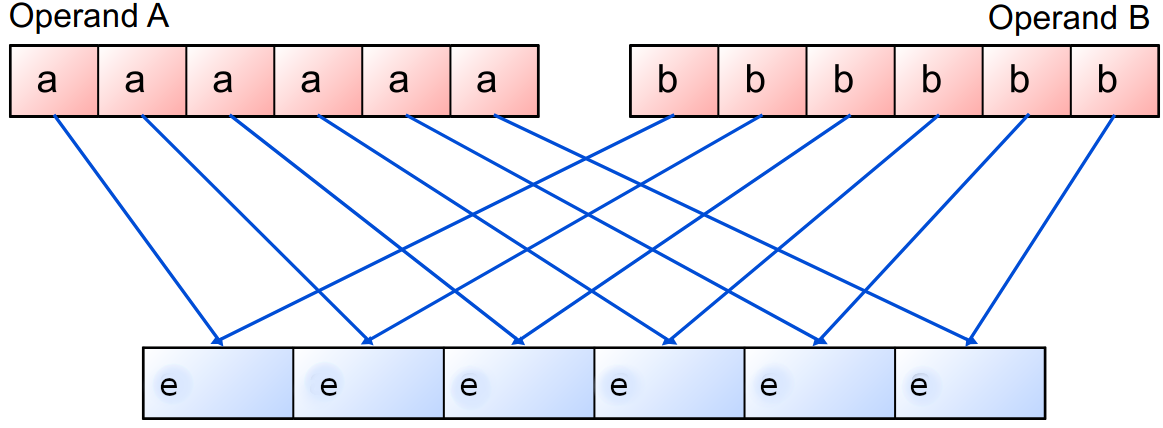
\includegraphics[scale=0.3]{pictures/bitvec}
\end{figure}
Dann erhalten wir als Ergebnis: $E = A \circ B$
\end{center}
\end{frame}

\subsection{Bitmaskierung}
\begin{frame}{Bitmaskierung}
\begin{center}
UND, ODER und XOR als spezielle Bit-Masken
\begin{figure}
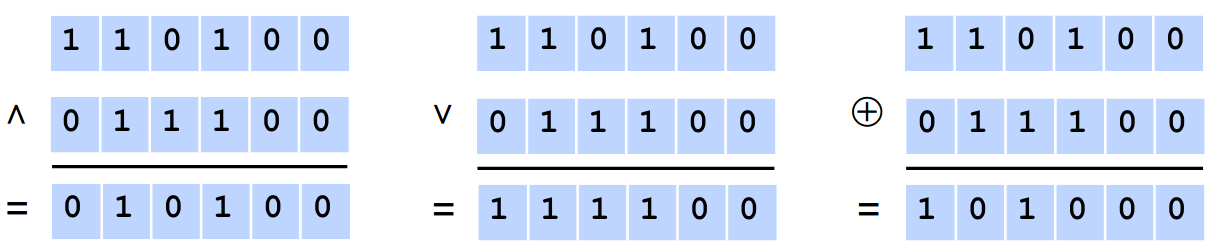
\includegraphics[scale=0.35]{pictures/masking}
\end{figure}
\end{center}
\end{frame}

\begin{frame}{UND Maskierung}
Maskierung von IP-Adressen:
\begin{figure}
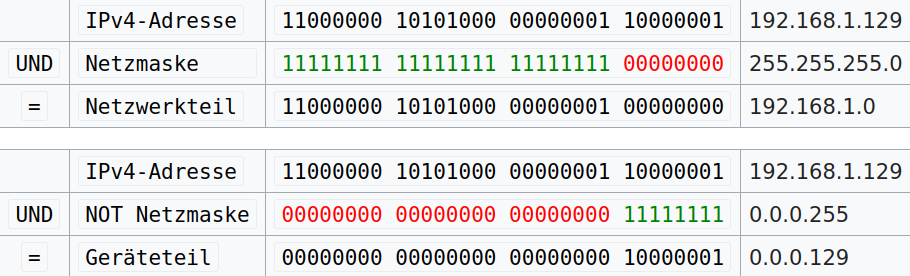
\includegraphics[scale=0.4]{pictures/UND}
\end{figure}
\end{frame}
\begin{frame}{OR Maskierung}

\begin{center}
Image Mask
\begin{figure}
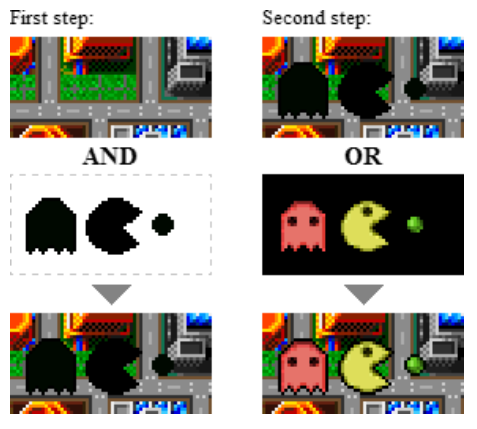
\includegraphics[scale=0.4]{pictures/OR}
\end{figure}
\end{center}
\end{frame}



\section*{Quellen}
\appendix
\begin{frame}[allowframebreaks]
  \frametitle<presentation>{Quellen}
\printbibliography
\end{frame}
\end{document}